\documentclass[aspectratio=169]{beamer}
\setbeamertemplate{navigation symbols}{}
\usepackage{color,amsmath,comment, subfigure}
\usepackage{booktabs}
\usepackage{url}

\def\imagetop#1{\vtop{\null\hbox{#1}}} %http://tex.stackexchange.com/questions/23521/tabular-vertical-alignment-to-top

%\setbeameroption{show notes}

%%%%%%%%%%%%%%%%%%%%%%%%%%
\title[]{Class 16: Experimental studies of contagion}
\author[]{Matthew J. Salganik}
\institute{Sociology 204: Social Networks\\Princeton University}
\date[]{
Pre-read video
\vfill

\begin{flushleft}
\vspace{0.6in}

\includegraphics[width=0.1\textwidth]{figures/cc.png}
\end{flushleft}
}

%%%%%%%%%%%%%%%%%%%%%%%%%%%
% SWBAT Describe the challenge of isolating contagion from other causes of similarity
% SWBAT Describe different designs to measure social contagion
% SWBAT Use ideas of internal validity and external validity to identify concerns with experiments
% SWBAT TODO
%%%%%%%%%%%%%%%%%%%%%%%%%%%%%%%%%%%%%%%%%%
\begin{document}
\frame{\titlepage}
%%%%%%%%%%%%%%%%%%%%%%%%%%%
\begin{frame}

\begin{itemize}
\item ``birds of a feather flock together'' but why? \pause
\item Experiments are powerful ways to isolate and estimate causal effects \pause
\item Experiments are powerful but not perfect: internal validity, external validity, and ethics 
\end{itemize}

\end{frame}
%%%%%%%%%%%%%%
\begin{frame}

People are often similar to the people they are connected to socially\pause
\begin{itemize}
\item selection (like people become friends) \pause
\item shared environment \pause
\item contagion
\end{itemize}
\vfill
\pause
For some traits, selection dominates (e.g., gender). \pause For other traits, all might be at work.
\end{frame}
%%%%%%%%%%%%%%%%%%%%
\begin{frame}

\begin{itemize}
\item ``birds of a feather flock together'' but why? 
\item \textcolor{blue}{Experiments are powerful ways to isolate and estimate causal effects}
\item Experiments are powerful but not perfect: internal validity, external validity, and ethics 
\end{itemize}

\end{frame}
%%%%%%%%%%%%%%
\begin{frame}

``It's like you don't harass women, you don't steal, and you've got to have a control group. This is one of the things that you can lose your job for at Harrah's not running a control group.''
Gary Loveman, CEO Harrah's

\end{frame}
%%%%%%%%%%%%%%%%%%%%%%%%%%
\begin{frame}

Notice how both papers describe that it is hard to make causal claims about contagion.  Part of the contribution of each paper is to bring experimental evidence.  You will see two \textit{field} experiments.

\end{frame}
%%%%%%%%%%%%%%%%%%%%%%%%%%%%
\begin{frame}

\begin{center}
\only<1>{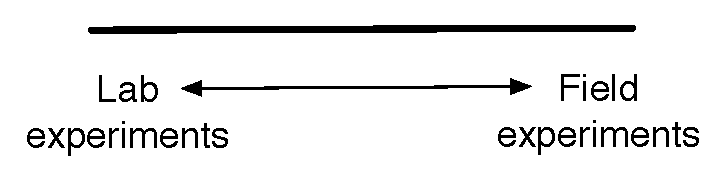
\includegraphics[width=0.7\textwidth]{figures/experiments_design_space_1d.pdf}}
\only<2>{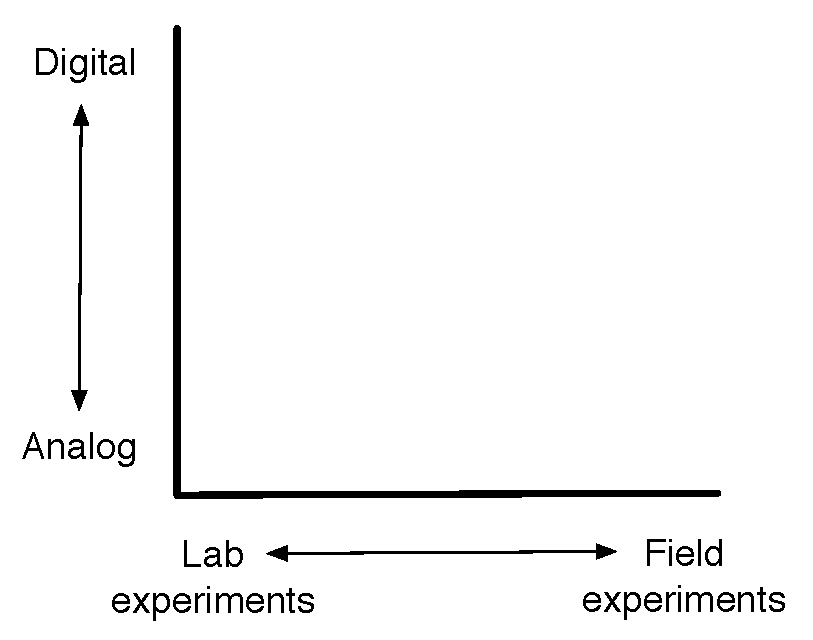
\includegraphics[width=0.7\textwidth]{figures/experiments_design_space_2d.pdf}}
\end{center}

\end{frame}
%%%%%%%%%%%%%%%%%%%%%%%
\begin{frame}

Experiments have four main ingredients:
\begin{itemize}
\item recruiting participants \pause
\item randomization treatment \pause
\item delivering treatment and control \pause
\item measuring outcomes 
\end{itemize}

\end{frame}
%%%%%%%%%%%%%%%%%%%%%%%%
\begin{frame}

Notice how both experiments put a lot of care into creating the control group.

\end{frame}
%%%%%%%%%%%%%%%%%%%%%%
\begin{frame}

A note on terminology:\\
Perturb and observe experiments vs randomized controlled experiments

\end{frame}
%%%%%%%%%%%%%%%%%%%%%%%%%%
\begin{frame}

These experiments move from the individual to the dyad.

\begin{center}

\includegraphics[width=0.2\textwidth]{figures/point}
\end{center}

\pause

\begin{center}
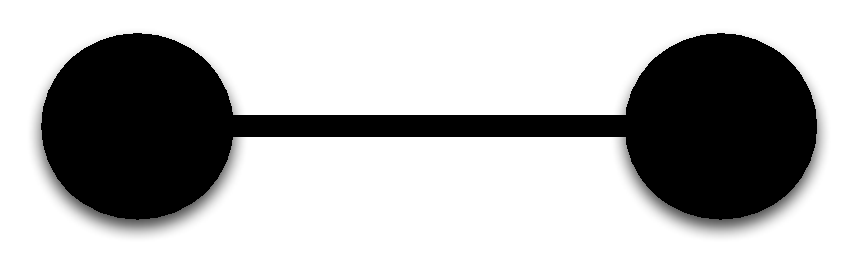
\includegraphics[width=0.5\textwidth]{figures/dyad}
\end{center}

\end{frame}
%%%%%%%%%%%%%%%%%%%%
\begin{frame}

\begin{itemize}
\item ``birds of a feather flock together'' but why? 
\item Experiments are powerful ways to isolate and estimate causal effects
\item \textcolor{blue}{Experiments are powerful but not perfect: internal validity, external validity}
\end{itemize}

\end{frame}
%%%%%%%%%%%%%%%%%%%%%%%%%%%%%%%%%
\begin{frame}

\begin{itemize}
\item Internal validity: were the experimental procedures performed correctly? \pause
\item External validity: what does this experiment tell us about this phenomena more broadly?
\end{itemize}

\vfill
For more information see Chapter 4 of Bit by Bit: \url{https://www.bitbybitbook.com/en/1st-ed/running-experiments/}

\end{frame}
%%%%%%%%%%%%%%%%%%%%%%%%%%%%%%%%%
\begin{frame}

\begin{itemize}
\item ``birds of a feather flock together'' but why? 
\item Experiments are powerful ways to isolate and estimate causal effects
\item Experiments are powerful but not perfect: internal validity, external validity
\end{itemize}

\vfill
I hope that helps provide some context for the readings

\end{frame}


\end{document}
